% Originally: content/week-07.tex, \section{Tangent and normal spaces} (Corsin Week 7)

% Source: Corsin Nick/Class Notes/Week 7.pdf, pp. 7--8
\section{Tangent and normal spaces}
\label{sec:tangent_normal_spaces}

\subsection{Tangent space}

Suppose $M^m \subseteq \mathbb{R}^n$ is a submanifold and $f : U \to f(U) \subseteq M$ is a local
parametrization around some point $p \in f(U)$ with $f(q) = p$. The $n\times m$ matrix
\[\Jac f(q) = \begin{pmatrix} \dfrac{\partial f}{\partial q_1} & \cdots & \dfrac{\partial f}{\partial q_m} \end{pmatrix}\]
has full rank, that is, the column vectors $\partial_if(q)$ are linearly independent. They form a
basis of $T_pM$:

% Sonnet 5 (Medium) --- FIG-W07-04
\begin{center}
\begin{tikzpicture}[>=Latex, scale=1.1]
  % A wireframe surface patch (parallel curve families) with a marked point p
  \foreach \i in {0,0.6,...,2.4} {
    \draw[blue!40!black, thin] plot[smooth] coordinates
      {(-1.4+\i*0.15,-1.1+\i*0.25) (-0.5+\i*0.15,-0.3+\i*0.25) (0.6+\i*0.15,0.1+\i*0.25) (1.6+\i*0.15,-0.2+\i*0.25)};
  }
  \foreach \j in {0,0.55,...,2.2} {
    \draw[blue!40!black, thin] plot[smooth] coordinates
      {(-1.4+\j*0.15,-1.1+\j*0.05) (-0.6+\j*0.35,-0.55+\j*0.15) (0.3+\j*0.55,-0.1+\j*0.2) (1.3+\j*0.7,0.05+\j*0.2)};
  }
  \coordinate (P) at (0.1,-0.05);
  \fill (P) circle (1.7pt) node[below, font=\small] {$p = f(q)$};
  \draw[orange!90!black, thick, ->] (P) -- ++(1.1,0.35)
    node[right, font=\scriptsize] {$\partial f/\partial x_1$};
  \draw[purple, thick, ->] (P) -- ++(0.35,0.95)
    node[above, font=\scriptsize] {$\partial f/\partial x_2$};
\end{tikzpicture}
\end{center}

\begin{definition}[Tangent space]
\label{def:tangent_space}
For $M$, $f$ as above, the \newterm{tangent space} \germanfor{Tangentialraum} of $M$ at
$p \in M$ is
\[T_pM := \operatorname{span}\{\partial_1f(q),\dots,\partial_mf(q)\} = Df_q(\mathbb{R}^m);\]
it is independent of the choice of $f$.
\end{definition}

\begin{example}[Tangent space to the upper hemisphere]
Parametrize the upper hemisphere $S^2_+ := \{(x,y,z)\in\mathbb{R}^3 : x^2+y^2+z^2=1,\ z>0\}$
graphically, i.e.,
\[f(x,y) = \begin{pmatrix} x \\ y \\ \sqrt{1-x^2-y^2} \end{pmatrix}.\]
We determine $T_{e_3}S^2_+$, where $e_3 = (0,0,1)$:
\begin{align*}
\left.\frac{\partial f}{\partial x}\right|_{(x,y)=(0,0)}
  &= \left.\begin{pmatrix} 1 \\ 0 \\ \dfrac{-x}{\sqrt{1-x^2-y^2}}\end{pmatrix}\right|_{(x,y)=(0,0)}
   = \begin{pmatrix}1\\0\\0\end{pmatrix} = e_1, \\[1ex]
\left.\frac{\partial f}{\partial y}\right|_{(x,y)=(0,0)}
  &= \left.\begin{pmatrix} 0 \\ 1 \\ \dfrac{-y}{\sqrt{1-x^2-y^2}}\end{pmatrix}\right|_{(x,y)=(0,0)}
   = \begin{pmatrix}0\\1\\0\end{pmatrix} = e_2.
\end{align*}
So, $T_{e_3}S^2_+ = T_{e_3}S^2 = \operatorname{span}\{e_1,e_2\} = \mathbb{R}^2\times\{0\}$.
\end{example}

% Source: Diego Torres Tejeda/Notes - 13.04 - Diego Torres Tejeda.pdf, p. 2
% Generator: Gemini 3.6 Flash (High)
\begin{example}[Tangent space to the 2-Torus]
\label{ex:torus_tangent_space}
Consider the 2-torus $\mathbb{T}^2 \subset \mathbb{R}^3$ parametrized by $\phi(t,\theta) : \mathbb{R}^2 \to \mathbb{R}^3$,
\[
\phi(t,\theta) := \begin{pmatrix} (R_1 + R_2 \cos\theta)\cos t \\ (R_1 + R_2 \cos\theta)\sin t \\ R_2 \sin\theta \end{pmatrix},
\]
where $R_1 > R_2 > 0$ are the major and minor radii. The partial derivatives of $\phi$ with respect to the angles $t$ and $\theta$ yield two linearly independent column vectors:
\[
\frac{\partial \phi}{\partial t} = \begin{pmatrix} -(R_1 + R_2\cos\theta)\sin t \\ (R_1 + R_2\cos\theta)\cos t \\ 0 \end{pmatrix}, \qquad
\frac{\partial \phi}{\partial \theta} = \begin{pmatrix} -R_2\sin\theta\cos t \\ -R_2\sin\theta\sin t \\ R_2\cos\theta \end{pmatrix}.
\]
By \cref{def:tangent_space}, at any point $p = \phi(t,\theta) \in \mathbb{T}^2$, the tangent space is the two-dimensional vector subspace
\[
T_p \mathbb{T}^2 = \operatorname{span}\left\{ \frac{\partial \phi}{\partial t}(t,\theta), \; \frac{\partial \phi}{\partial \theta}(t,\theta) \right\}.
\]
In particular, at the outer point $p_0 := (R_1+R_2, 0, 0)\transp$ (where $t = 0, \theta = 0$), we obtain $\frac{\partial \phi}{\partial t}(0,0) = (0, R_1+R_2, 0)\transp$ and $\frac{\partial \phi}{\partial \theta}(0,0) = (0, 0, R_2)\transp$, so $T_{p_0}\mathbb{T}^2 = \{0\} \times \mathbb{R}^2$.
\end{example}

% Sonnet 5 (Medium) --- FIG-W07-05
\begin{center}
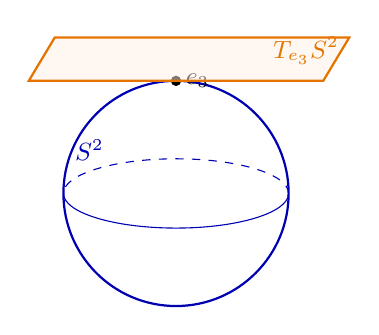
\begin{tikzpicture}[scale=1.1]
  \draw[blue!70!black, thick] (0,0) circle (1.3);
  \draw[blue!70!black, dashed] (1.3,0) arc (0:180:1.3 and 0.4);
  \draw[blue!70!black] (-1.3,0) arc (180:360:1.3 and 0.4);
  \node[blue!70!black, font=\small] at (-1.0,0.5) {$S^2$};

  \fill (0,1.3) circle (1.7pt) node[right, font=\small] {$e_3$};
  \draw[orange!90!black, thick, fill=orange!10, fill opacity=0.5]
    (-1.7,1.3) -- (1.7,1.3) -- (2.0,1.8) -- (-1.4,1.8) -- cycle;
  \node[orange!90!black, font=\small] at (1.5,1.65) {$T_{e_3}S^2$};
\end{tikzpicture}
\end{center}

% Quelle: Diego Torres Tejeda/Notes - 30.03 - Diego Torres Tejeda.pdf, p. 2 -- Sonnet 5 (Medium)
% Corsin defines T_pM only via a parametrization; the curve description below is Diego's. (Was
% an ainote until 2026-08-09. The mathematics is the proposition, and who-wrote-which-definition
% is editor-facing by Test 2 in style.md.)
\Cref{def:tangent_space} builds $T_pM$ out of a parametrization, so the space is pinned down by a
formula rather than by what its elements are. There is an equivalent description that says what
they are. A vector is tangent to $M$ at $p$ exactly when some curve running inside $M$ passes
through $p$ with that velocity, which is both how tangent vectors are usually pictured and the
quicker test in practice, since no parametrization need be written down.

\begin{proposition}[Tangent space via curves]
\label{prop:tangent_space_via_curves}
Let $M^m \subseteq \mathbb{R}^n$ be a $C^k$ submanifold ($k\geq1$) and $p \in M$. Then
\[T_pM = \big\{\gamma'(0) : \gamma \in C^1\big((-\varepsilon,\varepsilon), \mathbb{R}^n\big),\ \varepsilon>0,\ \gamma(t) \in M \text{ for all } t,\ \gamma(0)=p\big\}.\]
\end{proposition}

\begin{proof}
Let $\Phi : U \to V$ be a submanifold chart at $p$ (\cref{def:submanifold}), so
$\Phi(U\cap M) = (\mathbb{R}^m\times\{0\})\cap V$ and $\Phi(p)=0$; equivalently, let
$f := \Phi^{-1}|_{(\mathbb{R}^m\times\{0\})\cap V}$ be the corresponding local parametrization
(\cref{thm:local_parametrization}), $f(q)=p$.

\textbf{($\subseteq$)} Let $v \in T_pM = Df_q(\mathbb{R}^m)$, say $v = Df_q(w)$. The curve
$\gamma(t) := f(q+tw)$, defined for $t$ small enough that $q+tw$ stays in $f$'s domain, satisfies
$\gamma(t) \in M$ for all such $t$, $\gamma(0) = p$, and by the chain rule
$\gamma'(0) = Df_q(w) = v$.

\textbf{($\supseteq$)} Let $\gamma$ be a curve as in the statement. Since $\Phi$ is a
diffeomorphism with $\Phi(\gamma(t)) \in \mathbb{R}^m\times\{0\}$ for all $t$ near $0$, write
$\Phi\circ\gamma =: (\eta,0)$ with $\eta \in C^1\big((-\varepsilon,\varepsilon),\mathbb{R}^m\big)$.
Then $\gamma = \Phi^{-1}(\eta,0) = f(\eta(\cdot))$ near $0$ (shrinking $U$ if necessary so that
$f$ is defined on all of $\eta$'s image), so by the chain rule,
\[\gamma'(0) = Df_{\eta(0)}\big(\eta'(0)\big) \in Df_q(\mathbb{R}^m) = T_pM\]
(using $\eta(0)=q$, since $\Phi(p)=0=\Phi(f(q))$ and $\Phi$ is injective).
\end{proof}

% Sonnet 5 (Medium)
\begin{center}
\begin{tikzpicture}[>=Latex, scale=1.1]
  \draw[blue!70!black, thick] plot[smooth] coordinates
    {(-1.8,-0.8) (-0.8,0.6) (0.4,-0.2) (1.4,0.9) (2.2,0.1)};
  \coordinate (P) at (0.4,-0.2);
  \fill (P) circle (1.7pt) node[below, font=\small] {$p=\gamma(0)$};
  \draw[orange!90!black, thick, ->] (P) -- ++(0.9,0.75) node[right, font=\small] {$\gamma'(0)$};
\end{tikzpicture}
\end{center}

% Source: Jérôme Paschoud/Notizen/Woche 8.1 Tangentialräume und Jordan Mass.pdf, p. 1
% Generator: Gemini 3.1 Pro (High)
\begin{remark}[Four representations of the tangent space]
\label{rem:four_representations_tangent_space}
Depending on how a $m$-dimensional submanifold $M \subseteq \mathbb{R}^n$ is locally described near $p$, its tangent space $T_pM$ can be computed algebraically in four equivalent ways:
\begin{itemize}
  \item \textbf{Diffeomorphism} (from the definition, $\Psi(p)=0$): $T_pM = (D\Psi_p)^{-1}(\mathbb{R}^m \times \{0\})$.
  \item \textbf{Implicit representation} ($M = F^{-1}\{0\}$): $T_pM = \ker(DF_p)$.
  \item \textbf{Parametric representation} (local parametrization $g$ with $g(q)=p$): $T_pM = Dg_q(\mathbb{R}^m)$.
  \item \textbf{Graph representation} (graph of $h$, $p=(z, h(z))$): $T_pM = \{(w, Dh_z(w)) \mid w \in \mathbb{R}^m\}$.
\end{itemize}
These algebraic descriptions are all equivalent to the geometric description via velocities of curves (\cref{prop:tangent_space_via_curves}).
\end{remark}

\subsection{Normal space}

% Source: Corsin Nick/Class Notes/Week 7.pdf, pp. 9--10
Suppose $F : U \to \mathbb{R}^{n-m}$ is an implicit representation of $M^m = F^{-1}\{0\}$ (via the
regular value theorem) and $f : V^m \to M$ is a local parametrization, $M$ a submanifold. Then, by
definition,
\begin{enumerate}[label=\textbf{\arabic*.}]
  \item The Jacobian matrix:
\[ \Jac F(x) = \begin{pmatrix} \nabla F_1(x) \longrightarrow \\ \vdots \\ \nabla F_{n-m}(x) \longrightarrow \end{pmatrix} \]
    has full rank, i.e., $\{\nabla F_i(x)\}_{i=1,\dots,n-m}$ are linearly independent;
  \item $T_{f(q)}M = \operatorname{span}\{\partial_if(q)\}$, as above;
  \item $F(f(x)) = 0$ for all $x \in V$, since $f(x) \in M = F^{-1}\{0\}$.
\end{enumerate}
From \textbf{3}, it follows that
\begin{align*}
\Jac(F\circ f)(q)
  &= \Jac F(f(q))\cdot\Jac f(q) \\
  &= \begin{pmatrix} \nabla F_1(f(q)) \longrightarrow \\ \vdots \\ \nabla F_{n-m}(f(q)) \longrightarrow \end{pmatrix}
     \begin{pmatrix} \dfrac{\partial f}{\partial q_1} & \cdots & \dfrac{\partial f}{\partial q_m}\end{pmatrix}
   \;=\; 0.
\end{align*}
Now, since $\big(\Jac F(f(q))\cdot\Jac f(q)\big)_{ij} = \langle \nabla F_i(f(q)), \partial_jf(q)\rangle = 0$
for all $i=1,\dots,n-m$, $j=1,\dots,m$, the vectors $\nabla F_i(f(q))$ are perpendicular, that is,
\newterm{normal}, to $T_{f(q)}M$. Since by \textbf{1} we have $n-m$ linearly independent vectors
normal to the $m$-dimensional plane $T_{f(q)}M$, we can define:

\begin{definition}[Normal space]
\label{def:normal_space}
Let $M^m \subseteq \mathbb{R}^n$ be a submanifold and $F : U^n \to \mathbb{R}^{n-m}$ an implicit
representation, $M = F^{-1}\{0\}$. Then the \newterm{normal space} \germanfor{Normalraum} of
$M$ at $p \in M$ is
\[N_pM := \operatorname{span}\{\nabla F_1(p),\dots,\nabla F_{n-m}(p)\}.\]
\end{definition}

\begin{example}[Normal space to the sphere]
Represent $S^2$ implicitly: $S^2 = F^{-1}\{1\} = \{(x,y,z)\in\mathbb{R}^3 : F(x,y,z)=1\}$ where
$F(x,y,z) = x^2+y^2+z^2$. We determine $N_{e_3}S^2$:
\[\nabla F(0,0,1) = (2x,2y,2z)\big|_{(x,y,z)=(0,0,1)} = 2e_3.\]
So, $N_{e_3}S^2 = \operatorname{span}\{e_3\} = \{0\}\times\mathbb{R}$.
\end{example}

% Generator: Claude Opus 5 (High) --- the example above is the $n=3$, $F = \lvert x\rvert^2$
% instance of a general fact worth stating once, since it is what makes the Lagrange condition
% of \cref{prop:constrained_optimization} geometric rather than algebraic.
\begin{proposition}[The gradient is normal to the level set]
\label{prop:gradient_orthogonality_level_sets}
Let $U \subseteq \mathbb{R}^n$ be open, $g \in C^1(U,\mathbb{R})$, and let
$S := \{x \in U : g(x) = c\}$ for some $c \in \mathbb{R}$. If $\nabla g(x_0) \neq 0$ at a point
$x_0 \in S$, then near $x_0$ the set $S$ is an $(n-1)$-dimensional submanifold and
\[N_{x_0}S = \operatorname{span}\{\nabla g(x_0)\}.\]
In particular the normal space is a \emph{line}, and the affine \emph{tangent} hyperplane to $S$
at $x_0$ is $\{x \in \mathbb{R}^n : \langle x - x_0,\ \nabla g(x_0)\rangle = 0\}$.
\end{proposition}

\begin{proof}
That $S$ is a submanifold of dimension $n-1$ near $x_0$ is \cref{thm:regular_value_theorem},
since $\nabla g(x_0) \neq 0$ says exactly that $Dg_{x_0} : \mathbb{R}^n \to \mathbb{R}$ is
surjective. For the normal space, let $v \in T_{x_0}S$ and pick a $C^1$ curve
$\gamma : (-\varepsilon,\varepsilon) \to S$ with $\gamma(0) = x_0$ and $\gamma'(0) = v$. Then
$g \circ \gamma \equiv c$, so differentiating at $t=0$ with the chain rule along a path
(\cref{sec:chain_rule_along_path}) gives
\[0 = \frac{d}{dt}\Big|_{t=0}g(\gamma(t)) = \big\langle \nabla g(x_0),\ v\big\rangle.\]
Hence $\nabla g(x_0) \perp T_{x_0}S$, that is,
$\operatorname{span}\{\nabla g(x_0)\} \subseteq N_{x_0}S$. Both are subspaces of dimension
$n - \dim T_{x_0}S = n-(n-1) = 1$, so they are equal.
\end{proof}

% Supplement: Sascha Brack/Class Notes/Week_08_Notes_Monday.pdf, pp. 3--4
\begin{example}[Tangent and normal vectors via parametrization]
\label{ex:tangent_normal_parametrized_sphere}
For a parametrized surface $f : V \to \mathbb{R}^3$, the tangent space at $p = f(x)$ is $T_pM = \operatorname{span}\{\partial_1 f(x), \partial_2 f(x)\}$. A normal vector can be found via the cross product: $\vec{n} = \partial_1 f(x) \times \partial_2 f(x)$.

Let us apply this to the sphere $S^2$ using spherical coordinates:
\[\Phi(\theta,\varphi) = \begin{pmatrix} \sin\theta\cos\varphi \\ \sin\theta\sin\varphi \\ \cos\theta \end{pmatrix}, \qquad (\theta,\varphi) \in (0,\pi) \times (-\pi,\pi).\]
(Note that the image of $\Phi$ is the unit sphere minus a \qt{thin slice}, namely the meridian where $\varphi = \pm\pi$ together with the two poles where $\theta \in \{0,\pi\}$.)
The tangent space $T_{\Phi(\theta,\varphi)} S^2$ is spanned by the partial derivatives:
\[
\partial_\theta \Phi(\theta,\varphi) = \begin{pmatrix} \cos\theta\cos\varphi \\ \cos\theta\sin\varphi \\ -\sin\theta \end{pmatrix}, \qquad
\partial_\varphi \Phi(\theta,\varphi) = \begin{pmatrix} -\sin\theta\sin\varphi \\ \sin\theta\cos\varphi \\ 0 \end{pmatrix}.
\]
A normal vector is given by their cross product:
% Split across three lines: as one display this overflowed the text block by 70pt, which the
% house style forbids for chains of matrix blocks.
\begin{align*}
\vec{n} = \partial_\theta \Phi \times \partial_\varphi \Phi
  &= \begin{pmatrix} \cos\theta\cos\varphi \\ \cos\theta\sin\varphi \\ -\sin\theta \end{pmatrix}
     \times
     \begin{pmatrix} -\sin\theta\sin\varphi \\ \sin\theta\cos\varphi \\ 0 \end{pmatrix} \\
  &= \begin{pmatrix} \sin^2\theta\cos\varphi \\ \sin^2\theta\sin\varphi \\
       \sin\theta\cos\theta\cos^2\varphi + \sin\theta\cos\theta\sin^2\varphi \end{pmatrix} \\
  &= \sin\theta \begin{pmatrix} \sin\theta\cos\varphi \\ \sin\theta\sin\varphi \\ \cos\theta \end{pmatrix}.
\end{align*}
Its length is $|\vec{n}| = \sin\theta$ (since $\sin\theta > 0$ for $\theta \in (0,\pi)$).
The unit normal vector is therefore
\[
\nu(\theta,\varphi) := \frac{\vec{n}}{|\vec{n}|} = \begin{pmatrix} \sin\theta\cos\varphi \\ \sin\theta\sin\varphi \\ \cos\theta \end{pmatrix} = \Phi(\theta,\varphi).
\]
This confirms that the outward normal vector at a point on the unit sphere is precisely the position vector of that point.
\end{example}

% Sonnet 5 (Medium) --- FIG-W07-06
\begin{center}
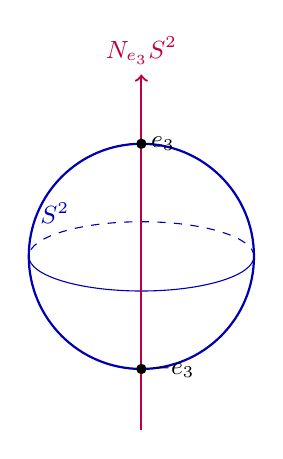
\begin{tikzpicture}[scale=1.1]
  \draw[blue!70!black, thick] (0,0) circle (1.3);
  \draw[blue!70!black, dashed] (1.3,0) arc (0:180:1.3 and 0.4);
  \draw[blue!70!black] (-1.3,0) arc (180:360:1.3 and 0.4);
  \node[blue!70!black, font=\small] at (-1.0,0.5) {$S^2$};

  \draw[purple, thick, ->] (0,-2.0) -- (0,2.1) node[above, font=\small] {$N_{e_3}S^2$};
  \fill (0,1.3) circle (1.7pt) node[right, font=\small] {$e_3$};
  \fill (0,-1.3) circle (1.7pt) node[right, font=\small] {$-e_3$};
\end{tikzpicture}
\end{center}


% --- exercise relocated here from the dissolved sheet 7 ---

% Originally: content/week-07.tex, \exercisesheet{7}, problem 7.6
% Source: exercises/Ex7_Analysis2_eng.pdf

\begin{exercise}[7.6 --- Spherical coordinates \textnormal{(important)}]
\label{ex:7.6}
The mapping $\Phi : (0,\infty)\times(0,\pi)\times(-\pi,\pi) \to \mathbb{R}^3$ defined by
\[\Phi(r,\theta,\varphi) = \begin{pmatrix} r\sin\theta\cos\varphi \\ r\sin\theta\sin\varphi \\ r\cos\theta \end{pmatrix}\]
is called \textit{spherical coordinates}.
\begin{enumerate}[label=\textbf{\arabic*.}]
  \item Sketch the images of $r \mapsto \Phi(r,\theta_0,\varphi_0)$, $\theta \mapsto
    \Phi(r_0,\theta,\varphi_0)$ and $\varphi \mapsto \Phi(r_0,\theta_0,\varphi)$ for some fixed
    $r_0 \in (0,\infty)$, $\theta_0 \in (0,\pi)$, $\varphi_0 \in (-\pi,\pi)$.
  \item What is the image of $\Phi$?
  \item Show that $\det(D_{(r,\theta,\varphi)}\Phi) = r^2\sin\theta$ holds.
  \item Conclude that the mapping $\Phi$ is a diffeomorphism onto its image.
\end{enumerate}
\end{exercise}
